\documentclass[10pt,a4paper]{article}
\usepackage{graphicx}
\usepackage{hyperref}
\usepackage[utf8x]{inputenc}

\begin{document}

\begin{titlepage}
\begin{center}


\includegraphics[scale=0.25]{../../common/sakuralogo.png}
\vfill

\huge
4MB PCMCIA SRAM

User's Manual

\vspace*{1cm}

\normalsize
Low cost Fast RAM expansion for Amiga 600/1200.

\vspace*{5cm}

\today

\end{center}
\end{titlepage}

\section*{Overview}

Thank you for purchasing Sakura 4MB PCMCIA SRAM expansion! This product has the following features:

\begin{itemize}
	\item Adds 4MB of Fast RAM to Amiga 600 or Amiga 1200.
	\item Accelerates unexpanded Amiga 1200 to at least 1.67 MIPS (according to SysInfo).
	\item Built using modern, high performance 55ns SRAM ICs.
	\item Very simple installation - just insert the card into PCMCIA slot on the left side of Amiga.
	\item Compatible with all PCMCIA friendly accelerators and memory expansions\footnote{We did our best to ensure that this card works on as many configurations as possible, but some accelerator and Fast RAM expansion designs are inherently incompatible with PCMCIA slot if more than 4MB of memory is installed. Note that PCMCIA SRAM should work with them anyway, if less than 4MB Fast was installed on the turbo card. Of course, if you don’t have any accelerator, you don’t have to worry about that.}.
	\item Open source design\footnote{Visit the source code reposity: \url{https://github.com/rkujawa/ppa-pcmcia-sram} .} under CC-BY-SA (board) and MIT (CPLD core) licenses.
	\item Made by Amigans for Amigans! 
\end{itemize}

\section*{Installation}

The installation process is very easy. To install the expansion perform the following steps:

\begin{itemize}
	\item Power down your Amiga.
	\item Slide the expansion card into PCMCIA slot, located on the left side of your computer. The card's components should be facing upwards.
	\item Be sure the {\tt RAM/disk} switch is in {\tt RAM} position.
	\item Turn on your Amiga and enjoy additional 4MB of memory.
\end{itemize}

Your Amiga should start as normal, albeit a bit faster. After installation you can confirm that the board is working correctly, by checking amount of available memory on the Workbench top menu bar, or with the {\tt avail} or {\tt ShowConfig} commands. Popular SysInfo tool will report the additional 4MB of memory under {\tt card.resource} name.

\section*{Technical details}

\begin{center}
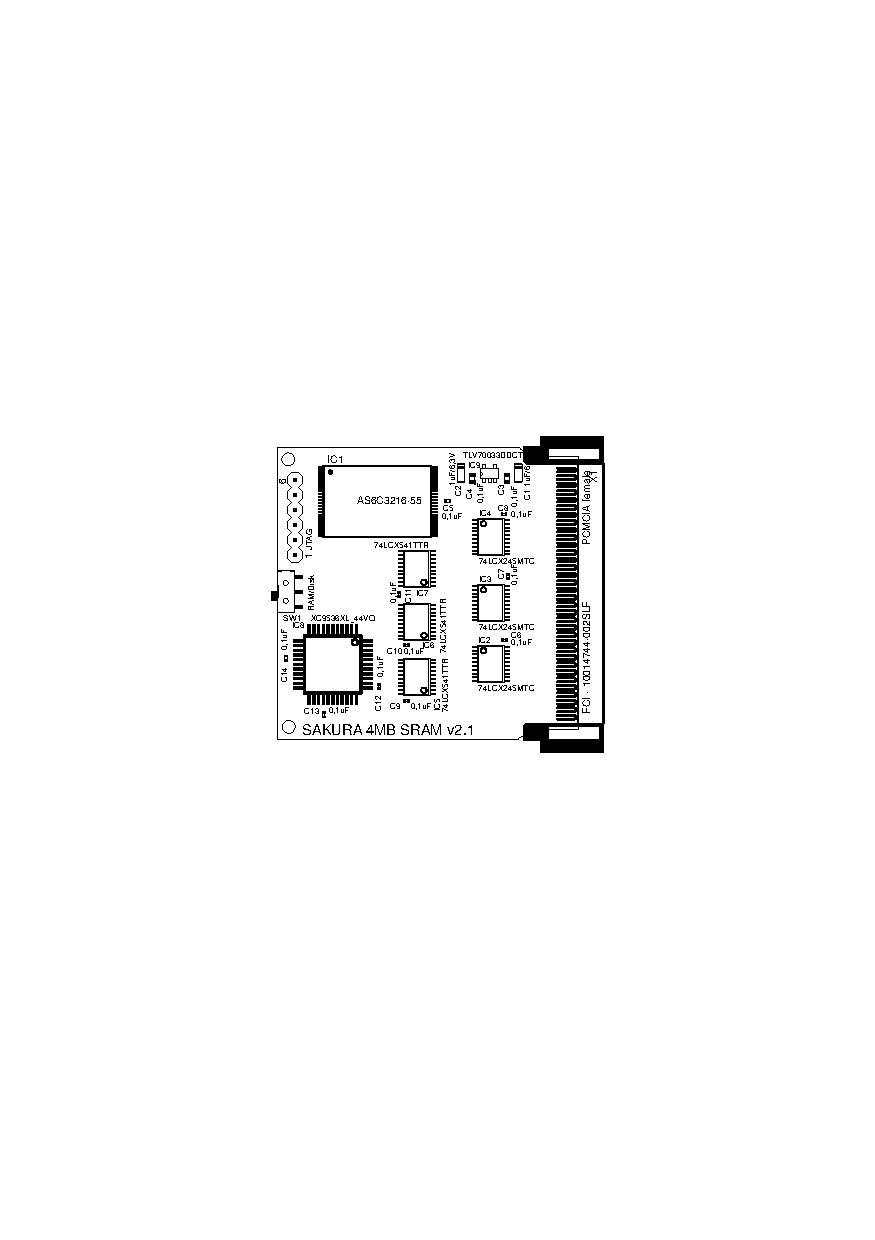
\includegraphics{board21layout.pdf}
\end{center}

Revision 2.x Sakura boards are built around Alliance Memory AS6C3216, which is a 55ns 32 megabit SRAM chip with 16-bit data bus. The memory is accessible within high 4MB of Zorro 2 memory ({\tt 0x600000-0x9FFFFF}) range.

Control signals for SRAM are generated by Xilinx XC9536XL CPLD, based on PCMCIA slot access signals.

This expansion is a completely autoconfiguring device. Memory is automatically added to the system memory pool by Kickstart. Autoconfiguration process is done according to the Card Information Structure (CIS) provided by the card, which is parsed by {\tt card.resource}. Naturally, this process only takes place during system startup, so inserting card into Amiga when it is running does not cause memory to be added. If necessary it could be added manually with {\tt AddMem} command (avaialble on aminet), although this is not required during normal operation.

Sakura expansion CIS contains optimal settings that allow best possible PCMCIA slot peformance:
\begin{itemize}
	\item On Amiga 600 Gayle chip is configured for 570ns access time by default, which results in performance similar to Fast RAM expansions attached on top of 68000 CPU.
	\item On Amiga 1200 the default configuration is 250ns access time, but Kickstart automatically reconfigures Gayle for 100ns access, according to CIS. This results in some performance increase compared to an unexpanded Amiga 1200. Contrary to popular opinions, Amiga 1200 equipped with high performance, correctly configured PCMCIA SRAM expansion (like this one) is performing better than Chip RAM only system.
\end{itemize}

CIS ROM is also implemented within XC9536XL CPLD.

Sakura expansion is electrically compatible with PCMCIA 2.1 standard, however physical dimensions of the card are smaller. While in theory this card should work with other devices, using it with computers other than Amiga 600/1200 was never tested and is discouraged.

\section*{Temporary disk mode}

It is possible to use the Sakura board as temporary virtual disk. To switch the board into this mode, take the following steps:
\begin{itemize}
	\item Turn off your Amiga and remove the Sakura board.
	\item Set the {\tt RAM/disk} switch into {\tt disk} position.
	\item Turn on your Amiga, instert the Sakura after booting into Workbench.
	\item Run the {\tt PrepCard} application.
	\item Select {\tt Prepare as disk} option.
	\item After your card is successfully prepared, reboot the Amiga.
	\item Notice the new volume named {\tt Empty} on your Workbench screen. Enjoy your temporary 4MB storage.

Card in this mode is handled by the device {\tt CC0}, which is provided by the Kickstart.
\end{itemize}

\section*{Troubleshooting}

\begin{itemize}
	\item Q: After powering up the Amiga, the memory does not appear on the Workbench bar and the output of {\tt ShowConfig} command.
	\item A: Check if the card is properly inserted into PCMCIA slot. Check if the {\tt RAM/Disk} switch is in the {\tt RAM} position. Reboot the Amiga.
\end{itemize}

\begin{itemize}
	\item Q: The memory is not automatically added to the system if Sakura card is inserted when Amiga is already powered on. 
	\item A: The probe procedure for PCMCIA memory is executed only during system startup. Reboot the Amiga to see the additional memory. 
\end{itemize}

\begin{itemize}
	\item Q: {\tt PrepCard} utility refuses to start, stating that memory is already configured. 
	\item A: It is not necessary to use {\tt PrepCard} with Sakura board configured as RAM. Predefined CIS settings are selected with {\tt RAM/Disk} switch. It is possible to view the current CIS settings by starting the {\tt PrepCard} just after inserting the card into Amiga (i.e. before reboot). 
\end{itemize}

\begin{itemize}
	\item Q: Performance of my Amiga 1200 dropped after installing the card.
	\item A: Be sure that {\tt RAM/disk} switch is in {\tt RAM} position. If not then turn off your Amiga completely, wait a few seconds and set the switch in {\tt RAM} position. After power-on you should notice considerable speedup.
\end{itemize}

\section*{Acknowledgements}

Sakura expansion was designed by Radosław ,,strim'' Kujawa and Jarosław ,,jarob'' Bieliński. The original idea was suggested on PPA.pl forum by RomanWorkshop. 

All schematics and board layout files are licensed under Creative Commons Attribution-ShareAlike 4.0 license. CPLD core source is licensed under MIT license.

The card is made in Poland and conforms to RoHS standard. 

All new cards sold through our exclusive dealer, RetroAmi, are covered by 24 months warranty. Due to open source nature of the project, note that {\bf only} cards produced by us (and therefore sold through RetroAmi) are covered by this warranty. In case of necessary service repairs please contact the shop directly. Do not attempt to repair the card yourself, it will void the warranty. Do not remove the sticker on the back of the card - it contains serial number. Please save the invoice/bill as a proof of transaction.

Thanks to everyone who preordered the board - you made this project happen!

\section*{Contact}

In case of any questions/inquires please contact RetroAmi:

\url{http://retroami.com.pl/} 

\end{document}

